\section{Implementation}

\begin{figure*}
  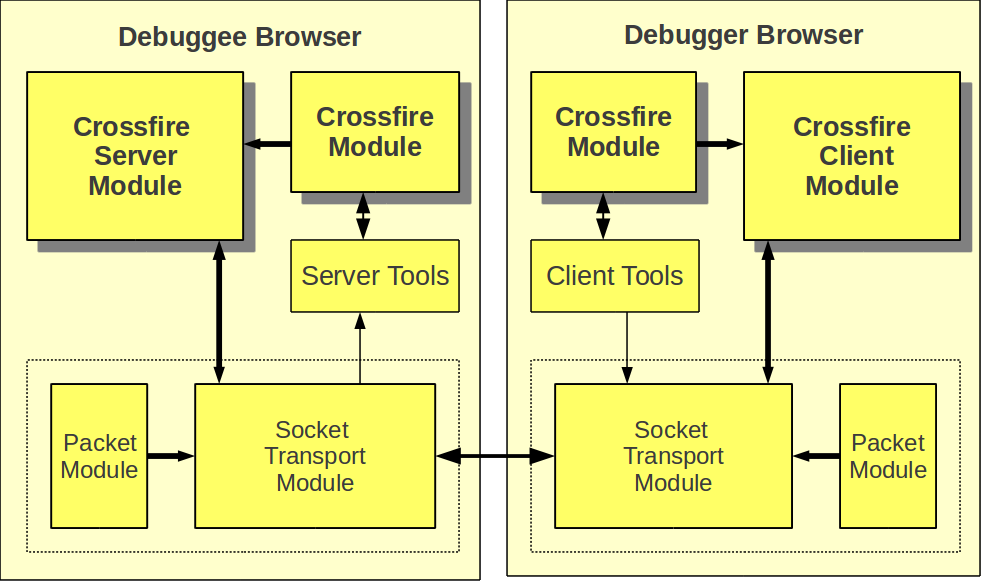
\includegraphics  [width = 86 mm] {figures/crossfire-arch4.png}
  \caption{Crossfire Firefox Extension Architecture}
 \label{fig:crossfire-arch}
\end{figure*}

\subsection{Crossfire Firefox Extension}
The first implementation of the Crossfire protocol is an extension implements
the protocol as an extension to Firefox and Firebug. This extension implements a
flexible transport layer, allowing the extension to operate as either a
Crossfire client or server. This will also enable both client and server to be
implemented on top of other transport layers, such as Web Sockets or HTTP.



\subsection{Crossfire Tools API}
The Crossfire extension also implements an API, called the ``Crossfire Tools API''
which enables extensibility of the Crossfire system and protocol. Firebug
features such as the Console, Inspector, and Net Panel, are implemented as tools
using the API.

\subsection{Modules}

\subsection {Browser Tools Interface}